\documentclass[prl,twocolumn]{revtex4-1}

\usepackage{graphicx}
\usepackage{color}
\usepackage{latexsym,amsmath}

\definecolor{linkcolor}{rgb}{0,0,0.65} %hyperlink
\usepackage[pdftex,colorlinks=true, pdfstartview=FitV, linkcolor= linkcolor, citecolor= linkcolor, urlcolor= linkcolor, hyperindex=true,hyperfigures=true]{hyperref} %hyperlink%



\begin{document}

\title{2216 -- Some catch title for the assignment}



\author{Ema Baci}
\author{Christoffer Askvik Faugstad}
\author{Melika Keshavarzmirzamohammadi}
\author{Veslemøy Therese Svendby Osmundsen}

\date{\today}


\begin{abstract}
An investigation was done to determine how different hyper parameters on a deep neural network impacts its performance. Architecture of the network, training parameters and initialization of the layers in the model was tuned by using grid search, yielding the best possible model for the task. It was found that a smaller sample size for training is sufficient to yield a good accuracy as long as the number of epochs is increased, and that in the case of limited data points, augmentation serves well as an artificial generator of more samples.
%Say something about architecture and other finds as well
\end{abstract}

\maketitle

\section{Introduction}
In this task a sequential deep neural network was built to perform binary classification. The aim was to predict whether a given point in a grid of size $\left[-50,50\right]$ was positioned within the boundaries of a chosen geometric shape.



\paragraph{\bf Tips}
\begin{itemize}
\item In English use sentences shorter than what you might normally be using in Italian, German, etc...
\item Possibly, Explain concepts at a level which is accessible to everybody.
\item Do not use colloquial forms in scientific writing, thus avoid it's, aren't, don't, etc.
\item Do not change the time of verbs; it is simpler to speak in simple present, however also writing always in past tense is fine.
\item In figures, use fonts that match the \underline{size} of the main text fonts (tiny fonts should be avoided). Use lines with different dashing, color, and symbol as appropriate for better distinguishing the curves. Use log scale when it is better for highlighting smaller scales or flattening larger scales. 
\item Remember the grid explained in the intro video of the course, which will be used for evaluations. It contains suggestions for improving the text.
\end{itemize}


%%%%%%%%%%%%%%%%%%%
\begin{figure*}[!tb]
  \centering
  \includegraphics[width=0.3\textwidth]{task_1/num_train_box.pdf}
  \hskip 1mm
  \includegraphics[width=0.3\textwidth]{task_1/num_train_box.pdf}
  \hskip 1mm
  \includegraphics[width=0.3\textwidth]{task_1/num_train_box.pdf}
  \vskip 1mm
  \includegraphics[width=0.455\textwidth]{task_1/num_train_box.pdf}
  \hskip 1mm
  \includegraphics[width=0.455\textwidth]{task_1/num_train_box.pdf}
  \caption{Description of the panels: (a)..... (b)... etc. This caption should give enough info on the content of figures to make them mostly readable without consulting the main text. However, repetitions with the main text should e avoided if possible. {\color{red} If this format is difficult to frame in the page you want, just break it into multiple single figures.}}
  \label{fig:x}
\end{figure*}
%%%%%%%%%%%%%%%%%%%

 \section{Methods}
\subsection{}


\subsection{General model}
The model is created by using Keras.Sequential(), which yields a fully connected deep neural network. The hidden layers are of the type Dense, with the activation function and number of nodes as inputs. A dropout layer was added to prevent biased weights, and the sigmoid function is given as activation in the final layer. The different parameters of the architecture is given by input to the compiler in order to apply grid search for tuning.
%Insert code of the model function

\subsection{Gridsearch}
There are many parameters to be determined within in a neural network. Grid search is an effective way of finding the optimal combination of hyper parameters and was the method used for the finetuning of our model. The parameters were divided into the three categories; arcitecture, training and initialization, and a grid search was done for each category.


\subsection{Initialization and activation functions}
The training of a neural network is very sensitive to its initial weights. In keras the default initialization of the initial weights is a glorot uniform distribution. The glorot uniform distribution is specially designed for the sigmoid function, and draws values uniformly from the interval $-[\textrm{limit},\textrm{limit}]$, where the limit depends on the number of input and output layers. The formula of the limit is given by 

\begin{equation}
    \textrm{lim}_\textrm{Glorot} = \sqrt{\frac{6}{\textrm{fan}_{in}+\textrm{fan}_{out}}},
\end{equation}

where $\textrm{fan}_{in}$ and $\textrm{fan}_{out}$ denotes the number of input and output layers respectively. However, the glorot initialization is not necessarily the best option for the rectified linear unit activation function which is also frequently used in neural networks. The limits of the He uniform distribution is given as
\begin{equation}
    \textrm{lim}_\textrm{He} = \sqrt{\frac{6}{\textrm{fan}_{in}}},
\end{equation}
depending only on the number of input layers. This is normally a better option for the rectified linear unit activation function. Both distributions were tested to initialize the weights of our model. The activation functions that are tested are sigmoid, relu, and elu, shown respectively as
\begin{equation}
    \sigma(x) = \frac{1}{1+e^{-x}}
    \label{eq:sigmoid}
\end{equation},
\begin{equation}
    f_\textrm{relu}(x) = \max \{0,x\}
    \label{eq:relu}
\end{equation} 
and 
\begin{equation}
    f_\textrm{elu}(x) = \begin{cases}
    x, \ \ \ \ \ \ \ \, x \geq 0\\
    e^x -1, \ x < 0
    \end{cases}
    \label{eq:elu}
\end{equation}


\subsection{Augmenting data}
The data is augmented by adding a small number $\epsilon$ to each of the variables. The $\epsilon$ is drawn uniformly from $[-5\cdot10^2,5\cdot10^2]$.


\subsection{Variations in the training set}
The performance as a function of the number of samples was investigated by having a fixed architecture and optimization procedure while varying the number of data samples used for training. 

\subsection{Grid search for architecture}
A grid with varying number of nodes, number of layers, dropout rate and hidden layer activation function was done, using cross validation.  

\subsection{Grid search for training}



\begin{table}[!b]
\begin{center}
\begin{tabular}{ll}
quantity & value \\
\hline
initial activation function & relu \\
hidden layers activation function & relu\\
final activation function & Sigmoid \\
number of hidden layers & $4$ \\
number of nodes hidden layers & $10$\\
dropout & $0.0$\\
optimizer & adam\\
epochs & $200$ \\
batch size & 16\\
training samples & 3200\\
validation samples & 800\\
target function & triangle
\end{tabular}
\end{center}
\caption{The default parameters used for the network architecture and its training parameters.}
\label{tab:optimal_value}
\end{table}

 
 
\begin{table}[!b]
\begin{center}
\begin{tabular}{llllll}
\hline
accuracy & time[s] & layers & nodes & dropout & afunc \\
\hline
0.92 (0.05) & 10 (2) & 4 & 10 & 0.0 & relu\\
0.92 (0.05) & 10 (2) & 3 & 40 & 0.1& relu\\
\hline
\end{tabular}
\end{center}
\caption{The best architectures found from grid search with cross validation. Time is the time average time used to train the network. Layers is the number of hidden layers. Nodes are the number of nodes in each hidden layer. Dropout is the dropout rate of the nodes in the hidden layers. Afunc is the activation function used in the hidden layers.}
\label{tab:grid_search_architecture}
\end{table}

\section{Results}


Describe what you found.

Cite Figure~a), etc. to add information. Later also cite Figure~ and  Figure~. Of course the number and size of figures may vary from project to project.

Cite Table~\ref{tab:1} to collect useful data in a clear way.

\subsection{Variations in the training set}

From figure \ref{fig:num_train_samples} there is a clear correlation between number of training samples and the average accuracy. The increased accuracy approach the optimal value. There is also a smaller spread in the obtained accuracies as the number of training samples increases. From the data one can conclude that $3200$ training is a satisfactory compromise between accuracy and computation time. The larger values of training samples has the same similar average, but considerably less variation. 


\subsection{Augmented data}
The accuracy's obtain over 10 runs, each with different proportions of augmented data compared to real data. \ref{fig:augmented_train_sampels}. The figure shows that adding extra augmented samples decrease the average accuracy, but at the expense of this the spread of the data is smaller.


\begin{figure}[ht]
  \includegraphics[width=0.44\textwidth]{num_train_box.pdf}
  \caption{The accuracy's achieved by the default network with a varying number of training samples. Each started from 10 different initial weights.}
  \label{fig:num_train_samples}
\end{figure}


\begin{figure}[!tb]
  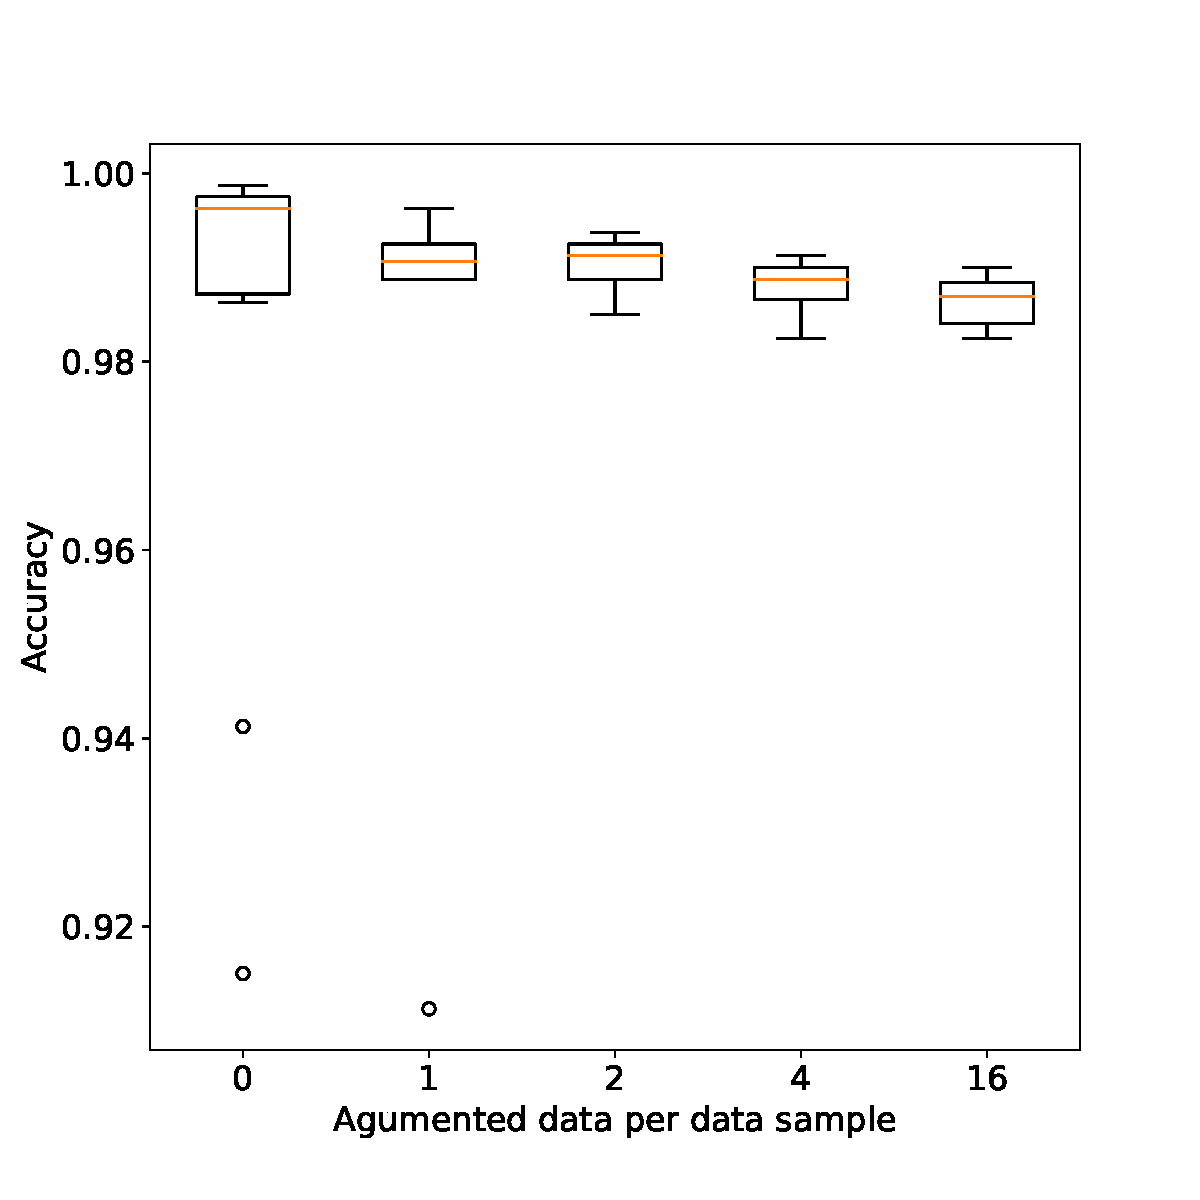
\includegraphics[width=0.44\textwidth]{ag_train_box.pdf}
  \caption{The different accuracy's achieved by the default network when adding the indicated number of augmented data per original training data. The values are for 10 different initial weights for each augmented data per original training data. The original training data consist of $3200$ samples.}
  \label{fig:augmented_train_sampels}
\end{figure}


\section{Conclusions}

Discuss the key aspects that we can take home from this work.

Check if your text is light, swift, and correct in exposing its passages.





\begin{thebibliography}{99}

\bibitem{pap1}
  B. Franklin,
  J. Here There {\bf 10}, 20--40 (1800).
  
\bibitem{pap2}
  A. Einstein,
  Int. J. There Here {\bf 20}, 125--133 (1910).
  
\end{thebibliography}

\clearpage

% %%%%%%%%%%%%%%%%%%%
% \begin{figure*}[!tb]
%   \centering
%   \includegraphics[width=\textwidth]{description_assignment_LCPB_20-21.pdf}
% \end{figure*}
% %%%%%%%%%%%%%%%%%%%


\end{document}
















% Templates that might be needed


\begin{table}[!b]
\begin{center}
\begin{tabular}{lll}
quantity & symbol & dimensionless \\
\hline
time & $t$ & $t'$  \\
momentum & $p$ & $v$
\end{tabular}
\end{center}
\caption{Description of the table.}
\label{tab:1}
\end{table}














